\documentclass[12pt,a4paper]{article}
\usepackage[utf8]{inputenc}
\usepackage[T2A]{fontenc}
\usepackage[russian,english]{babel}
\usepackage{amsmath}
\usepackage{amsfonts}
\usepackage{amssymb}
\usepackage{graphicx}
\usepackage[left=2cm,right=2cm,top=2cm,bottom=2cm]{geometry}
\usepackage{calc}
\usepackage{setspace}
\usepackage{indentfirst}
\usepackage{caption}
\usepackage{xcolor}
\usepackage[unicode]{hyperref}
\usepackage{minted}

\definecolor{codebg}{rgb}{0.96,0.96,0.96}  % светлый фон
\definecolor{textcolor}{rgb}{0.1,0.1,0.1}   % тёмный текст

\setminted{
    bgcolor=codebg,
    fontsize=\small,
    breaklines=true,
    frame=lines,
    framesep=2mm,
    baselinestretch=1.2,
    encoding=utf8
}

\usemintedstyle{tango}  % стиль с хорошей контрастностью


% Стиль для C++
\newminted{cpp}{
    commentstyle=\color{gray},  % серые комментарии
    keywordstyle=\color{blue!70!black},  % тёмно-синие ключевые слова
    stringstyle=\color{red!70!black},     % тёмно-красные строки
    identifierstyle=\color{textcolor},    % основной текст
    numberstyle=\color{gray!60},          % номера строк
    showspaces=false,
    showtabs=false
}

% Стиль для NASM
\newminted{nasm}{
    commentstyle=\color{gray},          % серые комментарии
    keywordstyle=\color{blue!70!black}, % тёмно-синие ключевые слова
    stringstyle=\color{red!70!black},   % тёмно-красные строки
    identifierstyle=\color{textcolor},  % основной текст
    numberstyle=\color{gray!60},        % номера строк
    showspaces=false,
    showtabs=false,
    linenos=true,
    numbersep=5pt,
    morekeywords={
        section,global,extern,equ,times,
        db,dw,dd,dq,resb,resw,resd,resq,
        mov,push,pop,call,ret,jmp,jz,jnz,je,jne,
        add,sub,mul,div,inc,dec,
        eax,ebx,ecx,edx,esi,edi,esp,ebp,
        rax,rbx,rcx,rdx,rsi,rdi,rsp,rbp
    }
}

% Стиль для Bash
\newminted{bash}{
    commentstyle=\color{gray},          % серые комментарии
    keywordstyle=\color{blue!70!black}, % тёмно-синие ключевые слова
    stringstyle=\color{red!70!black},   % тёмно-красные строки
    identifierstyle=\color{textcolor},  % основной текст
    numberstyle=\color{gray!60},        % номера строк
    showspaces=false,
    showtabs=false,
    linenos=true,
    numbersep=5pt,
    morekeywords={
        if,then,else,fi,for,while,do,done,
        case,esac,function,select,until,
        echo,export,read,printf,test,
        cd,ls,mkdir,rm,cp,mv,chmod,chown,
        grep,awk,sed,find,ssh,scp
    }
}

\title{
    Отчет о выполнении лабораторной работы 3565.32.50494452
    
    Оценка эффективности SIMD-оптимизаций программы Mandelbrat2
    }
    
\author{Швабра Владимир Сергеевич, Б01-411}

\captionsetup[figure]{name=Рис.}

\begin{document}
\maketitle

\newpage

\tableofcontents

\newpage

\section{Аннотация}
\subsection{Цели работы}  
\begin{enumerate}
    \item Научиться применять различные низкоуровневые оптимизации на примере расчёта множества Мандельброта.
    \item Научиться оценивать эффективность работы программы
\end{enumerate}

\subsection{Теоретическая справка}

Сначала рассмотрим базовую последовательную модель выполнения инструкций (SEQ), а затем перейдем к современным конвейерным реализациям (PIPE) с предсказанием переходов.

\subsubsection{Последовательная модель выполнения (SEQ)}
На рисунке \ref{fig:seq} представлена последовательная модель обработки инструкций:

\begin{figure}[ht!]
\centering
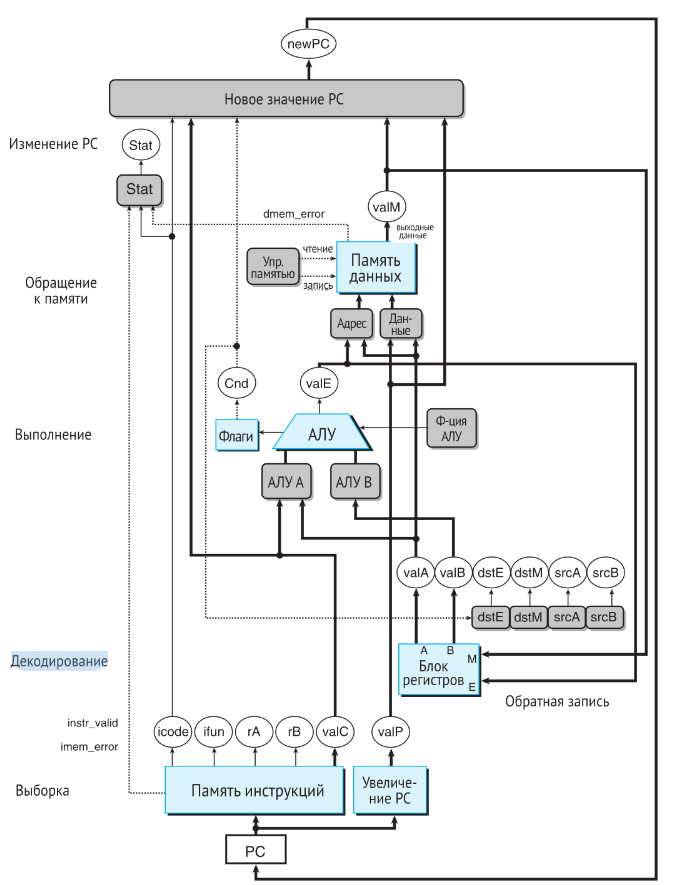
\includegraphics[width=0.9\textwidth]{seq.png}
\caption{Блок-схема последовательной обработки инструкций (SEQ)}
\label{fig:seq}
\end{figure}

\paragraph{Этапы последовательной обработки}

\begin{enumerate}
    \item \textbf{Выгрузка (F)}:
    \begin{itemize}
        \item Извлекает инструкцию из памяти по адресу, указанному в Program Counter (PC)
        \item Используется \textit{кэш инструкций} для ускорения доступа
        \item PC увеличивается на размер инструкции (или изменяется для инструкций перехода)
    \end{itemize}

    \item \textbf{Декодирование (D)}:
    \begin{itemize}
        \item Определяется \textit{тип операции} (арифметическая, логическая, перехода и т.д.)
        \item Выявляются \textit{операнды} (регистры, непосредственные значения, адреса памяти)
        \item Для операций с памятью вычисляются эффективные адреса
        \item Подготавливаются сигналы управления для следующих этапов
    \end{itemize}

    \item \textbf{Выполнение (E)}:
    \begin{itemize}
        \item Выполнение арифметических или логических операций в \textit{АЛУ} (Арифметико-Логическом Устройстве)
        \item Для условных переходов - проверка условий и вычисление адреса перехода
    \end{itemize}

    \item \textbf{Обращение к памяти (M)}:
    
    Этот этап присутствует только для инструкций работы с памятью.
    \begin{itemize}
    \item Для загрузки: чтение данных из памяти по вычисленному адресу
    \item Для записи: запись данных в память по вычисленному адресу
    \item Используется \textit{кэш данных} для ускорения доступа
    \item Обработка кэш-промахов и обращение к основной памяти при необходимости
    \end{itemize}

    \item  \textbf{Обратная запись (W)}:
    \begin{itemize}
        \item Для арифметических операций - запись в регистр-приемник
        \item Для операций загрузки - запись данных из памяти в регистр
    \end{itemize}

    \item \textbf{Изменение PC}:
    \begin{itemize}
        \item Для обычных инструкций: PC уже был увеличен на этапе выгрузки
        \item Для инструкций перехода: PC изменяется на новое значение
        \item Для условных переходов: PC изменяется только если условие истинно
        \item Обработка исключений и прерываний также может изменить PC
    \end{itemize}
\end{enumerate}

\paragraph{Ограничения SEQ}
Главный недостаток последовательной модели — низкая эффективность. Каждый этап задействует только часть аппаратных ресурсов процессора, остальные простаивают.

\subsubsection{Конвейерная модель выполнения (PIPE)}
Современные процессоры используют конвейерную обработку, как показано на рисунке \ref{fig:pipe}.

\begin{figure}[ht!]
\centering
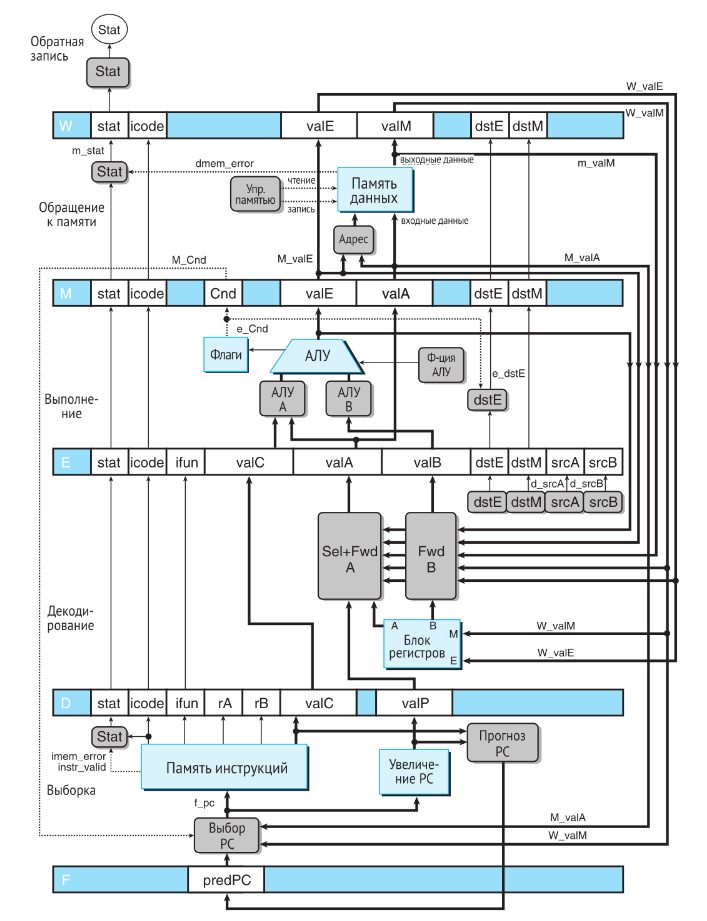
\includegraphics[width=0.8\textwidth]{pipe.png}
\caption{Блок-схема конвейерной обработки инструкций (PIPE)}
\label{fig:pipe}
\end{figure}

Из общих изменений в схеме добавились конвейерные регистры между каждой соседней парой этапов обработки инструкций. Это сделано для возможности выполнения разных этапов разных инструкций параллельно, как показно на рисунке \ref{fig:pipeline}.

\begin{figure}[ht!]
    \centering
    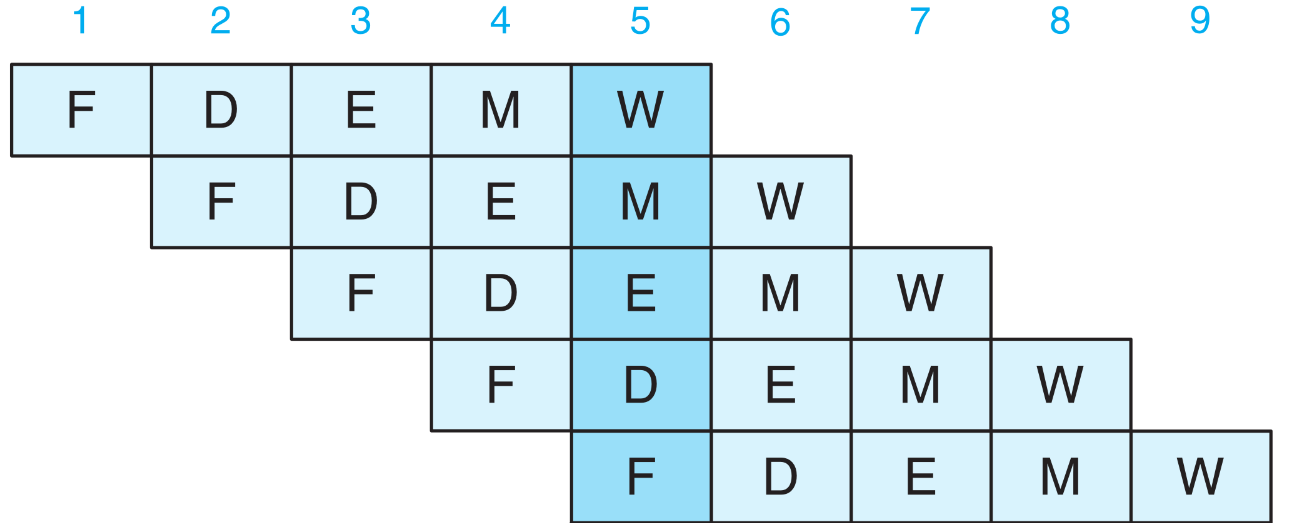
\includegraphics[width=0.8\textwidth]{pipeline.png}
    \caption{Визуализация конвейерной обработки инструкций}
    \label{fig:pipeline}
\end{figure}

\paragraph{Предсказание РС}
\indent

Если обрабатываемая инструкция не является условным переходом, то мы можем однозначно определить следующее значение PC, но иначе нет.

\begin{itemize}
    \item \textbf{Инструкции не выполняющие "прыжок" - } так как мы знаем размер каждой инструкции, то можем прибавить его к PC.
    \item \textbf{CALL, JMP, RET - } мы знаем адрес, на который нужно перейти \textit{в любом} случае.
    \item \textbf{Условный переход - } До проверки условия мы не знаем куда надо делать "прыжок".
\end{itemize}

Проблему с условными переходами можно решить приостановкой загрузки новых инструкций в конвейер до момента вычисления условия, но есть решение лучше. Мы попробуем угадать произойдёт переход или нет и продолжать подгружать операции с соответствующего места, а в случае ошибочного предсказания сбросить загруженные инструкции, что, конечно, ударит по производительности.

Существует много различных стратегий для предсказания переходов, но мы не будем в это углубляться. Отметим лишь, что для облегчения работы предсказателю, не стоит писать сложных условий без необходимости. Также нужно знать об операциях условного перемещения, которые могут улучшить производительность ветвлений.

\paragraph{Риски по данным}
\indent 

Но схема на рисунке \ref{fig:pipeline} будет работать корректно только если во всех инструкциях, которые выполняются параллельно не будет \textit{зависимости по данным}, что может часто не соблюдаться. Приведём методы разрешения таких зависимостей.

\begin{itemize}
    \item \textbf{NOP:} самое лёгкое решение. На этапе генерации ассемблера проставить пустые инструкции в количестве необходимом, для такого чтобы устранить параллельное выполнение инструкций зависимых по данным (Рис. \ref{fig:nop}).
    \begin{figure}[ht!]
        \centering
        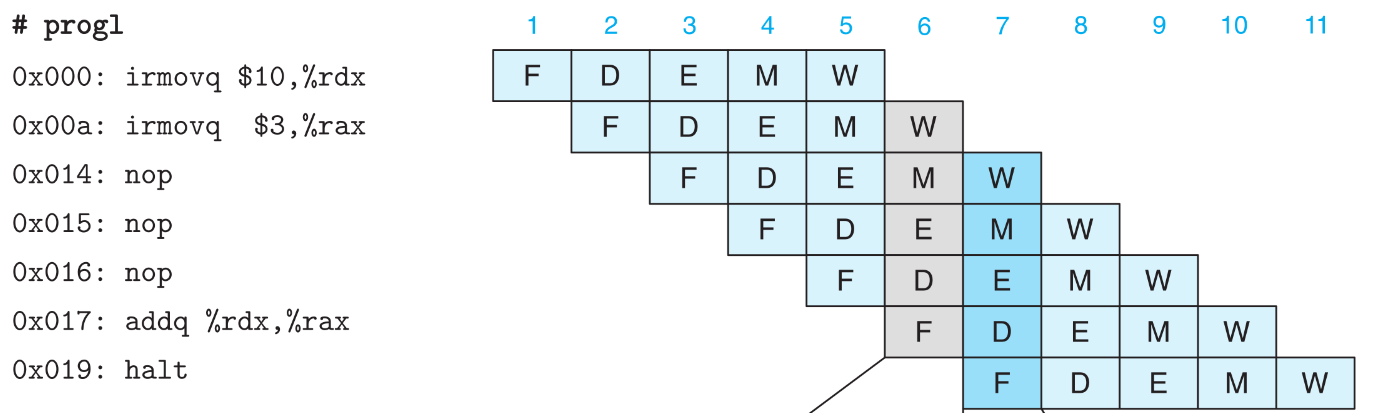
\includegraphics[width=0.8\textwidth]{nop.png}
        \caption{Останова, реализованная через NOP для решения проблемы риска по данным}
        \label{fig:nop}
    \end{figure}

    \item \textbf{"Пузырёк" (Привет дед!): } Аппаратная приостановка конкретных этапов обработки инструкций, зависящих по данным (Рис. \ref{fig:babble}).
    \begin{figure}[ht!]
        \centering
        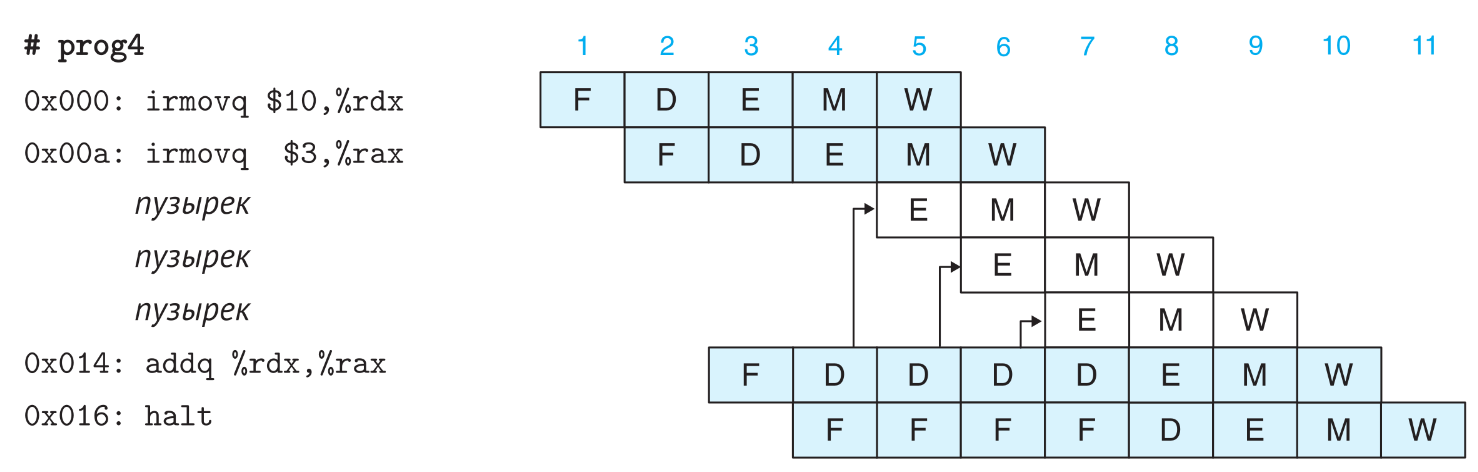
\includegraphics[width=0.8\textwidth]{babble.png}
        \caption{Останова, реализованная через "пузырёк" для решения проблемы риска по данным}
        \label{fig:babble}
    \end{figure}

    \item \textbf{Продвижение: } Мы добавляем в нашу конструкцию процессора (Рис. \ref{fig:pipe}) возможность передачи значений (регистров, либо памяти) в предыдущие этапы обработки инструкций, чтобы ожидающая инструкция могла использовать уже вычисленное значение до окончания обработки ожидаемой инструкции.
\end{itemize}

\paragraph{Взаимосвязь функциональных блоков}
\indent

В настоящих процессорах, очевидно, есть несколько функциональных блоков, каждый из которых занимается обработкой операций того или иного типа. Это позволяет выполнять некоторые операции не по порядку. Такая архитектура процессора называется суперскалярной (Рис \ref{fig:superscalar}) и хорошо дополняет конвейерное устройство функциональных блоков.

Распределением инструкций по функциональным блокам занимается \textit{блок управления инструкциями (БУИ (это я ввёл сам, так не называют, просто чтобы меньше писать (лисп сосать (дед упрлс (а стоп, это же не гайд на летку (ну ладно, пока (швабра)))))))}. В частности на всех современных процессорах есть блок для обработки ветвлений, который пытается предсказать условные переходы (аналогично предсказателю PC в рамках одного конвейера, но на уровень выше). Такая организация обработки инструкций называется \textit{спекулятивным выполнением}.

\begin{figure}[ht!]
    \centering
    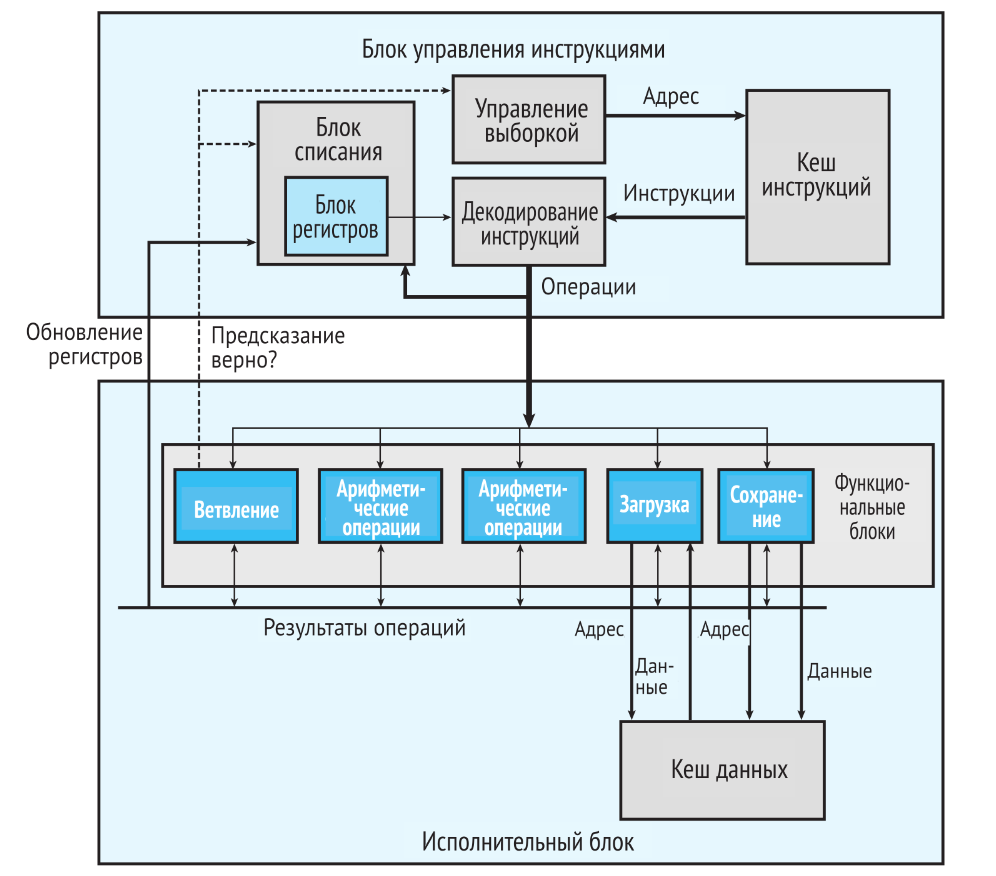
\includegraphics[width=0.8\textwidth]{supscalar.png}
    \caption{Блок-схема суперскалярного процессора}
    \label{fig:superscalar}
\end{figure}


\subsubsection{Оптимизации}

На основе знаний изложенных выше мы можем "класть" наш код на аппаратуру применением низкоуровневых оптимизаций, чтобы увеличить производительность. Некоторые из них мы сейчас опишем


\paragraph{Вынос кода}

Если в цикле вычисляется значение переменной и не меняется на всех итерациях цикла, то для данного значения стоит завести константу вне цикла и использовать её. Аналогично можно поступить при постоянном обращении к памяти, правда это будет эффективно в случае, если есть свободные регистры для сохранения переменной.

\newpage

\begin{minted}{cpp}
// До оптимизации
for (size_t i = 0; i < n; ++i) {
    double result = sin(x) * arr[y] + i;  // sin(x) и arr[y] не зависят от i
    printf("%f\n", result);
}

// После оптимизации
double sin_x = sin(x);
double arr_y = arr[y];
for (size_t i = 0; i < n; ++i) {
    double result = sin_x * arr_y + i;
    printf("%f\n", result);
}
\end{minted}

\paragraph{Уменьшение рисков по данным}

Стоит уметь представлять в голове как конвейерная и суперскалярная архитектура будут обрабатывать инструкции и минимизировать простои процессора. Допустим, если есть возможность переставить вычисление независимых операций, то их можно поставить между зависимыми, чтобы занять неиспользуемое время.

\begin{minted}{cpp}
// До оптимизации
float x = y * z;  // Независимая операция
float a = b * c;
float d = a + e;  // Зависит от a

// После оптимизации
float a = b * c;
float x = y * z;   // Независимая операция
float d = a + e;
\end{minted}

\paragraph{Комбинация развёртывания цикла и аккумулятора}
\indent

\textbf{Развёртывание: } это преобразование программы, которое уменьшает количество итераций за счет увеличения количества вычислений в каж­дой итерации. Развертывание цикла может улучшить производительность по двум причинам. Во-первых, уменьшается количество операций, не влияющих непосредственно на результат программы, таких как вычисление индекса и условное ветвление. Во-вторых, открываются возможности для дальнейшего преобразования кода при помощи аккумуляторов.

\textbf{Аккумуляторы: } Для ассоциативной и коммутативной комбинирующей операции (например для целочисленного сложения или умножения) производительность можно повысить, разбив набор комбинирующих операций на две или более частей, и комбинировать их результаты в конце. 

Без учёта накладных расходов использование описанных подходов можно увеличить скорость выполнения цикла во столько раз, на сколько порядков проведено развёртывание. Конечно, это можно делать не бесконечно, ведь в какой-то момент регистров для аккумуляторов не будет хватать и они будут сохраняться в переменные, что только замедлит обработку инструкций. Подробную оценку производительности читайте в БХ (байт для будущих пекусов).

\begin{minted}{cpp}
// До оптимизации
float sum = 0;
for (int i = 0; i < n; i++) {
    sum += array[i];
}

// После оптимизации (развёртывание 4x + аккумуляторы)
float sum0 = 0, sum1 = 0, sum2 = 0, sum3 = 0;
for (int i = 0; i < n; i += 4) {
    sum0 += array[i];
    sum1 += array[i+1];
    sum2 += array[i+2];
    sum3 += array[i+3];
}
float sum = sum0 + sum1 + sum2 + sum3;
\end{minted}

\paragraph{Применение векторных инструкций (SIMD)}

Модель выполнения инструкций SIMD позволяет производить одну операцию сразу с несколькими данными в соответствующих функциональных блоках с поддержкой векторных операций. Использование таких инструкций очень хорошо сочетается с вышеперечисленными оптимизациями.

\begin{minted}{cpp}
#include <immintrin.h>

// До оптимизации
for (int i = 0; i < n; i++) {
    c[i] = a[i] + b[i];
}

// После оптимизации
for (int i = 0; i < n; i += 4) {
    __m128 va = _mm_load_ps(&a[i]);
    __m128 vb = _mm_load_ps(&b[i]);
    __m128 vc = _mm_add_ps(va, vb);
    _mm_store_ps(&c[i], vc);
}
\end{minted}

\subsubsection{Измерение эффективности}

Наиболее точным способом измерения времени работы программы является ассемблерная инструкция \textit{rdtsc}, которая возвращает количество пройденных тактов с момента запуска программы. Проблема состоит в том, что тактовая частота при нормальной работе машины постоянно меняется. Мы можем зафиксировать её специальными утилитами (далее для ОС Fedora).

\begin{minted}{bash}
    # Установка нужных инструментов
    $ sudo dnf install kernel-tools cpupowerutils

    # Вывод информации о процессоре
    $ cpupower frequency-info
    analyzing CPU 0:
    #...
    hardware limits: 400 MHz - 3.60 GHz
    #...
    current CPU frequency: 2.23 GHz (asserted by call to kernel)
    #...
    # Несколько раз потыкав внешнюю программу можно понять какую максимальную частоту можно поставить, чтобы она не менялась. Я выбрал 1 GHz

    $ sudo cpupower frequency-set -u 1.0GHz

    # Проверям
    $ cpupower frequency-info

\end{minted}

После работы возвращаем всё на свои места, ставя ограничение на максимальную частоту больше, чем может быть максимум

\begin{minted}{bash}
    $ sudo cpupower frequency-set -u 3.6GHz
\end{minted}

Стоит уточнить, что измерение будет производиться на одном и том же "месте" множества мандельброта и при одинаковых параметрах экрана, чтобы расчёты были идентичными.

\section{Оборудование}

\begin{itemize}
    \item 2 банки энергетика
    \item конспекты деда
    \item 1 бутылка пива
    \item чипсы соседа
    \item третье издание БХ
    \item слинки (всем с СДВГ советую)
    \item ноутбук (опционально)
\end{itemize}

\section{Ход работы}

\subsection{Зависимости}

Для сборки проекта нужны Make и GCC. Для отрисовки множества Мандельброта возьмём библиотеку SDL2 (SFML для лохов), также дополнительно установим модуль TTF для вывода FPS на экран.

\subsection{Написание неэффективной версии}

В файле \texttt{mandelbrat2.c} первая реализация функции \verb|print_frame()| является неоптимизированной. Она нужна для проверки эффективности применённых оптимизаций, именно с ней мы и будем сравнивать итоговую версию. Для большей честности, код написан наиболее производительно, но без использования знаний об устройстве процессора и низкоуровневых оптимизаций.

В проекте написана обработка различных флагов, чтобы можно было изменять параметры отображения множества Мандельброта, отключать графику и увеличивать количество повторных обработок 1 кадра (для увеличения точности измерений).

Реализовано движение по множеству, а также приближение или отдаление к центру координат, чтобы было удобнее рассматривать математические красоты.

В правом верхнем углу экрана выводиться текущий FPS, чтобы примерно оценить скорость расчёта кадров, реализованный через функции SDL2.

\begin{figure}[ht!]
    \centering
    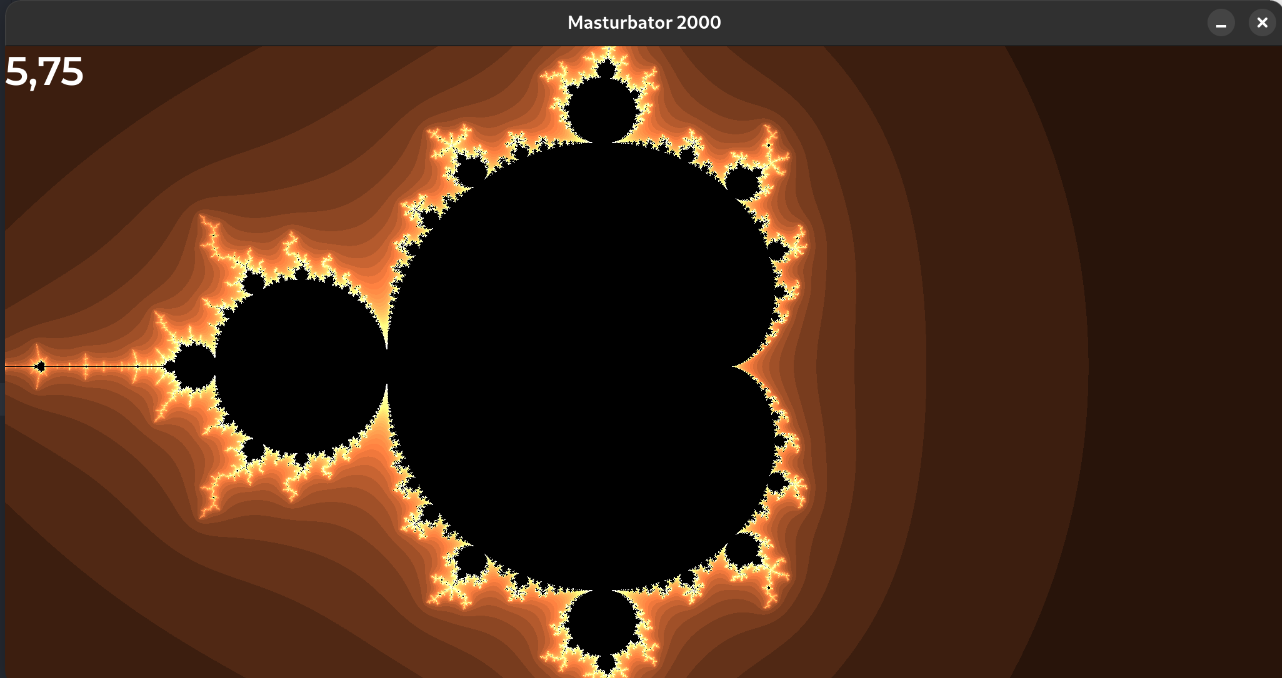
\includegraphics[width=0.8\textwidth]{mandlebrat_navx.png}
    \caption{Визуализация множества Мандельброта без оптимизаций}
    \label{fig:mandlebrat_navx}
\end{figure}

В среднем значение FPS варьируется от 5 до 6 на "дефолтной" позиции.

\subsection{Написание эффективной версии}

За основу возьмём алгоритм, описанный выше и изменим его. Сделаем вынос кода обращения к памяти и переставим инструкции, чтобы избавиться от зависимости по данным. В конце перепишем вычислительную часть через интрисинки, которые позволят обрабатывать сразу 4 double за 1 операцию.

% iters_cnt = 64
% r_circle_inf = 10
% scale = 550

% make USE_AVX2=1 ADD_FLAGS=-DSETTINGS_FILENAME='\"settings_avx.txt\"' OPTS="-r 50" DEBUG_=0 rebuild all 
% Time for calculate 1 frame: 4037358640966 tiks
% Time for calculate 2 frame: 8308478739 tiks
% Time for calculate 3 frame: 8454345726 tiks
% Time for calculate 4 frame: 8282673252 tiks
% Time for calculate 5 frame: 8353552892 tiks
% Time for calculate 6 frame: 8272863569 tiks
% Time for calculate 7 frame: 8306364832 tiks
% Time for calculate 8 frame: 8397524320 tiks
% Time for calculate 9 frame: 8288241897 tiks
% Time for calculate 10 frame: 8456685137 tiks
% Time for calculate 11 frame: 8373814372 tiks

% make USE_AVX2=0 ADD_FLAGS=-DSETTINGS_FILENAME='\"settings.txt\"' OPTS="-r 50" DEBUG_=0 rebuild all 
% Time for calculate 1 frame: 2545274689855 tiks
% Time for calculate 2 frame: 29492387584 tiks
% Time for calculate 3 frame: 29689503770 tiks
% Time for calculate 4 frame: 29648000294 tiks
% Time for calculate 5 frame: 29574279331 tiks
% Time for calculate 6 frame: 29564181810 tiks
% Time for calculate 7 frame: 29652688875 tiks
% Time for calculate 8 frame: 29547756022 tiks
% Time for calculate 9 frame: 29646507133 tiks
% Time for calculate 10 frame: 29706510410 tiks
% Time for calculate 11 frame: 29808649926 tiks




\section{Полезные ссылки}

\begin{itemize}
    \item \href{https://vk.com/wall-51126445_124413}{Компьютерные системы. Архитектура и программирование [2022] Брайант Р. Э., О'Халларон Д. Р.}
    \item \href{https://www.laruence.com/sse/#techs=MMX,SSE,SSE2,SSE3,SSSE3,SSE4_1,SSE4_2,AVX,AVX2&expand=4974,4923,3865,3869,3870,736&text=mul}{Зеркало сайта с интрисинками на intel}
    \item \href{https://github.com/kzueirf12345/mandelbrat2}{Сюда звёздочки ставить}
\end{itemize}


\end{document}